\chapter{Graph Theory}

\section{Basic concepts}

\subsection{Graph}

\begin{itemize}
\item A graph $G = (N, E)$ with $N$ a set of nodes and $E$ a set of edges, swhere an edge is a pair of two nodes.
\item Example : $N = {a, b, c}, E = {{a, b}, {b, c}}$
\end{itemize}

\subsection{Directed Graph}

\begin{itemize}
\item Each edge has a direction, and is represented as a tuple with a \textit{first} and a \textit{second}
\item Example : $E = {(a, b), (b, c)}$
\end{itemize}

\subsection{Undirected Graph}

\begin{itemize}
\item Edges have no direction, they are represented as a set
\item Example : $E = {{a, b}, {b, c}}$
\end{itemize}

\section{Paths and connectivity}

\subsection{Path}

A path in a graph is a sequence of nodes such that each successive pair in the sequence is an edge of the graph.

\subsection{Simple path}

A simple path is a path where each node occurs at most once.

\subsection{Cycle}

A cycle is a path with 3 or more edges such that the first and last nodes are the same and otherwise all node are distinct.

\subsection{Connected Graph}

A graph is connected if there exists a path between every pair of nodes.

\subsection{Component of a graph}

A component is a subset of nodes that satisfies two properties :
\begin{enumerate}
\item The subset is \textit{connected}.
\item The subset is \textit{maximal} : there is no superset that is connected.
\end{enumerate}

\subsubsection{Strongly connected component}

A component is strongly connected if it satisfies two properties :
\begin{enumerate}
\item Each node in the subset has a path to each other node in the subset.
\item The subset is \textit{maximal} : it is not part of a larger subset with the property that each node can reach the other.
\end{enumerate}

\subsection{Analyzing a graph}

\begin{itemize}
\item A graph can be divided into its components.
\item For each component, we can study its internal structure. For example, removing a node (with its edges) may split it in more components.
\end{itemize}

\subsection{Giant components}

Large social networks often have a giant component, which is a component that contains a significant fraction of the graph's nodes.

\subsection{Bipartite graph}

A bipartite graph is a graph where the nodes can be separated into two sets such that each edge connects a node from one set to the other.

\subsection{Clique or complete graph}

There exist an edge joining every pair of nodes.

\subsubsection{Labeled complete graph}

A complete graph where every edge is labeled.

\section{Distance in a graph}

\subsection{Length}

The length of a path is the number of edges it contains.

\subsection{Distance between two nodes}

Length of the shortest path between these two nodes.

\subsection{Breadth-first-search}

For finding distances between nodes.

\chapter{How to combine graph theory and sociology}

\section{Social networks}

A graph where the nodes denote human beings and the edges denote a connection between two human beings.

\subsubsection{Triadic closures}

\begin{figure}[H]
    \centering
    \includegraphics[width=0.4\textwidth]{triadic_closure}
\end{figure}

if two people in a social network have a common friend, then the likelihood that they will become friends in the future is increased :

\begin{itemize}
\item B and C have more opportunities to meet.
\item B and C both thrust A so they have a basis for trusting each other.
\item B and C have common interests with A so they may have common interests with each other.
\item A has an incentive to bring B and C together since if they are not friends, it stresses A.
\end{itemize}

\subsubsection{Strong triadic closure}

If A and B are close friends as well as A and C, then it is especially likely that B and C will become connected.

\subsection{Clustering coefficient}

\begin{figure}[H]
    \centering
    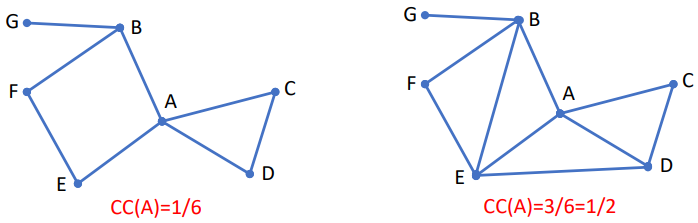
\includegraphics[width=0.5\textwidth]{clust_coef}
\end{figure}

The \textit{clustering coefficient} $CC(A)$ of node A in a graph is :
\begin{itemize}
\item $CC(A) =$ probability that two randomly selected friends of A are friends with each other.
\item $CC(A) = \frac{X}{Y}$
	\begin{itemize}
	\item $X =$ the number of pairs of A's friends that are connected.
	\item $Y =$ the maximum number of pairs of A's friends that are connected.
	\end{itemize}
\item Triadic closures causes the clustering coefficient to increase
\end{itemize}

\subsection{Bridges}

\begin{figure}[H]
    \centering
    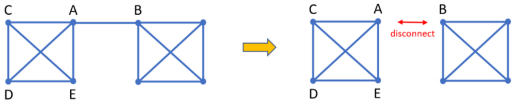
\includegraphics[width=0.5\textwidth]{bridge}
\end{figure}

The edge joining A and B is a \textit{bridge} if removing this edge causes A and B to be in different components.

\subsubsection{Local bridges}

\begin{figure}[H]
    \centering
    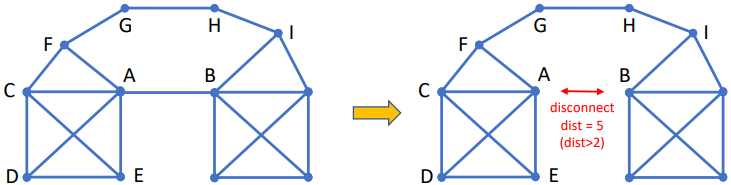
\includegraphics[width=0.5\textwidth]{local_bridge}
\end{figure}

\begin{itemize}
\item The edge joining A and B is a \textit{local bridge} if A and B have no friends in common, so deleting the edge will increase the distance between A and B to a value \textit{strictly greater than 2}.
\item Local bridges play roughly the same role as bridges, but in a less extreme way : they connect a node to another node that would otherwise be far away.
\end{itemize}

\subsection{Neighborhood overlap}

The neighborhood overlap generalizes local bridges :
$\frac{X}{Y}$ where
\begin{itemize}
\item $X =$ number of nodes who are neighbors of \textit{both} A and B.
\item $Y =$ number of nodes who are neighbors of \textit{at least one} of A and B.
\end{itemize}

\chapter{Networks in their surrounding context}

\section{Longitudinal studies}

The network must be followed over time.

\section{Homophily}

They are two basic mechanisms that cause friends to resemble each other : selection and social influence (both are sociological concepts)
\begin{itemize}
\item \textit{Selection} : people select friends with similar characteristics (an internal mechanism).
	\begin{itemize}
	\item individuals drive the formation of new links.
	\end{itemize}
\item \textit{Social influence} : people modify their behaviors to be closer to their friends (an external mechanism), also called "peer pressure".
	\begin{itemize}
	\item Existing links drive the formation of new links
	\end{itemize}
\end{itemize}

\subsection{Affiliation network}

\begin{figure}[H]
    \centering
    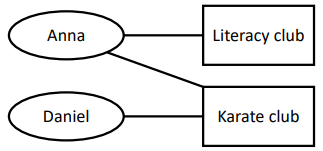
\includegraphics[width=0.35\textwidth]{affiliation_network}
\end{figure}

An affiliation network is a bipartite graph that shows which individuals are affiliated with which activities.
\begin{itemize}
\item The first set is the individuals.
\item The second set is the foci.
\end{itemize}

\subsubsection{Three forms of closures in a social-affiliation network}

\begin{figure}[H]
    \centering
    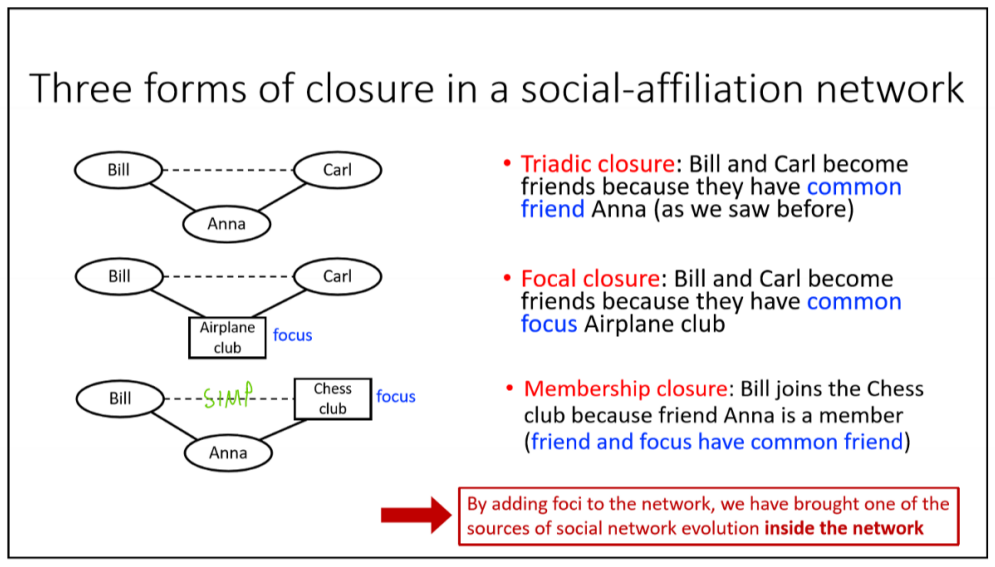
\includegraphics[width=0.7\textwidth]{closures_types}
\end{figure}

\subsection{Measuring homophily}

\begin{figure}[H]
    \centering
    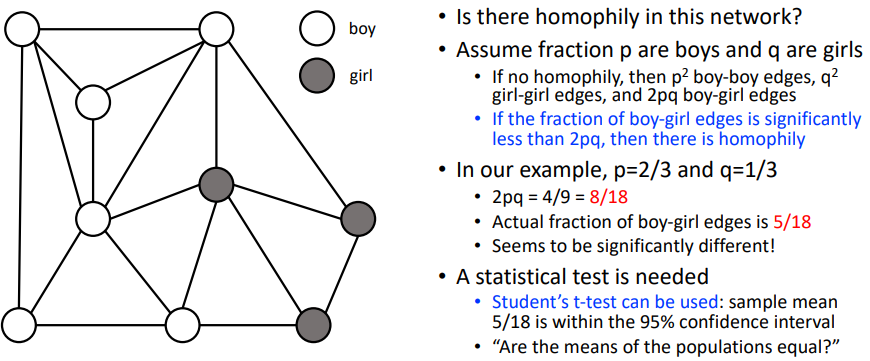
\includegraphics[width=0.8\textwidth]{homophilie_calc}
\end{figure}

\chapter{Positive and negative relationships}

\section{Structural balance}

\subsection{Balanced and unbalanced triangles}

\begin{figure}[H]
    \centering
    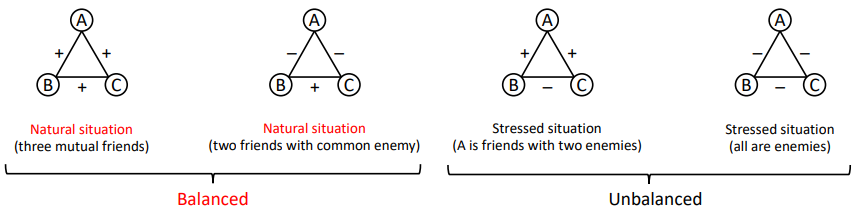
\includegraphics[width=0.6\textwidth]{balanced_unbalanced}
\end{figure}

\subsection{Balance for networks}

\subsubsection{Local definition}

A network is balanced if all the triangles in it are balanced

\subsubsection{Global definition}

If a labeled complete graph is balanced, then either all pairs of nodes are friends, or else the nodes can be divided into two groups such that nodes within a group are friends and nodes between groups are enemies.

\subsection{Weak structural balance}

\subsubsection{Local definition}

A network is balanced if all the triangles in it are balanced or they are (---).

\subsubsection{Global definition}

If a labeled complete graph is weakly balanced, then its nodes can be divided into groups such that any two nodes belonging to the same group are friends and any two nodes belonging to different groups are enemies.

\subsubsection{Degrees of structural balance}

\begin{figure}[H]
    \centering
    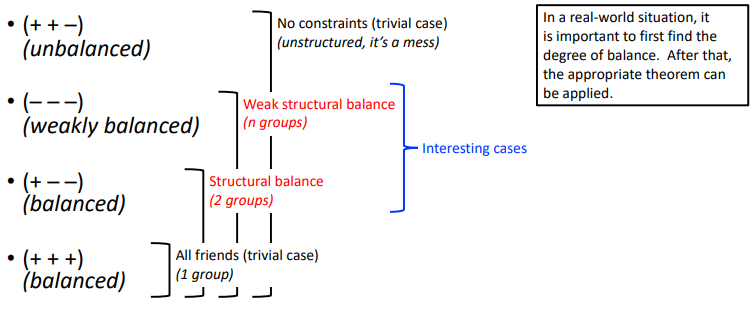
\includegraphics[width=0.6\textwidth]{degree_structural_balance}
\end{figure}

\chapter{Introduction to game theory}

Game theory studies the interaction of participants.

\section{Game with two rational player}

\subsection{Game}

\begin{itemize}
\item There is a set of participants, called the players.
\item Each player has a set of options for how to behave : we will refer to these options as the player's strategies.
\item For each choice of strategies (one by each player), each player receives a payoff. The payoff depends on the strategies selected by all players. Payoffs are generally numbers, and each player prefers larger payoffs to smaller ones.
\end{itemize}

\subsubsection{Assumptions}

\begin{enumerate}
\item All that a player care about is summarized in the payoff.
\item Each player knows everything about the game.
\item Each player chooses a strategy to maximize their own payoff, given a belied about the strategy ysed be the other player.
\end{enumerate}

\subsubsection{On shot game}

Two players that play only once and where the players simultaneously and independently choose their actions.

\subsubsection{Dynamic games}

Games that are played sequentially over time.

\subsubsection{Forms}

\paragraph{Normal form}

In normal form, each player commits ahead of time to a complete plan for playing the whole game.

\begin{figure}[H]
    \centering
    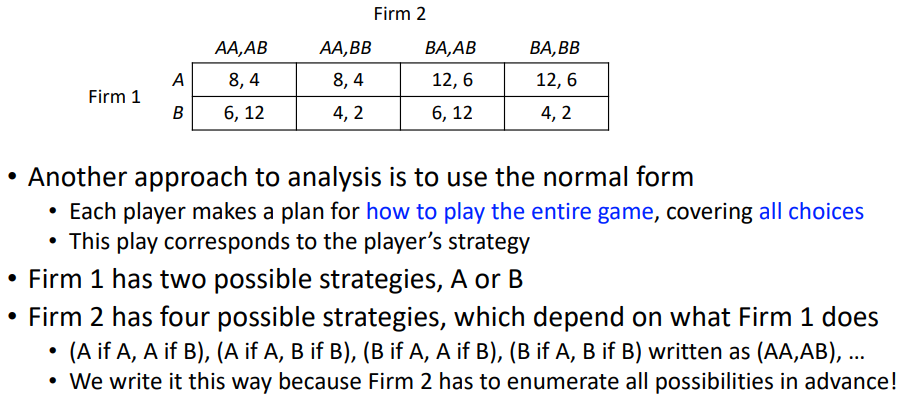
\includegraphics[width=0.6\textwidth]{normal_form}
\end{figure}

\paragraph{Extensive form}

In extensive form, each player makes an optimal decision at each intermediate step.

\begin{figure}[H]
    \centering
    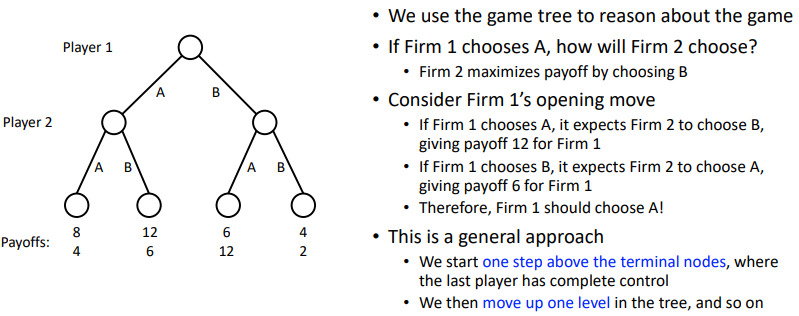
\includegraphics[width=0.7\textwidth]{extensive_form}
\end{figure}

\subsection{Strategies}

\subsubsection{Strictly dominant strategy}

When a player has a strategy strictly better than all others, regardless of what the other player does (not always possible).

\begin{table}[H]
    \centering
    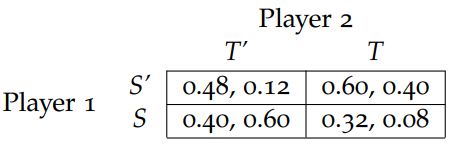
\includegraphics[width=0.35\textwidth]{strictly_dominant_strategy}
\end{table}

\subsubsection{Mixed strategies}

We introduce randomness.

\begin{table}[H]
    \centering
    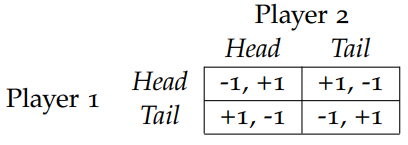
\includegraphics[width=0.35\textwidth]{mixed_strategies}
\end{table}

\subsubsection{Best response}

\begin{table}[H]
    \centering
    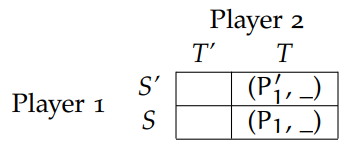
\includegraphics[width=0.25\textwidth]{best_response}
\end{table}

\begin{itemize}
\item S for player 1 is best response to T for Player 2 if :
	\begin{itemize}
	\item For all other strategies, $S'$ of Player 1 : $P1(S, T) \geq P1(S', T)$
	\end{itemize}
\item S for player 1 is strictly best response to T for Player 2 if :
	\begin{itemize}
	\item For all other strategies, $S'$ of Player 1 : $P1(S, T) > P1(S', T)$
	\end{itemize}
\end{itemize}

\subsubsection{Nash equilibrium}

\begin{itemize}
\item Each player's strategy is a best response to the other.
\item Corresponds to free market.
\end{itemize}

\begin{table}[H]
    \centering
    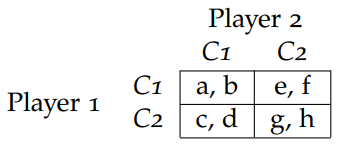
\includegraphics[width=0.28\textwidth]{nash_equilibrium}\\
    $P(C2, C1)$ is a Nash equilibrium if $a < c$ and $h < d$
\end{table}

\paragraph{Coordination / anti-coordination games}

Games with multiple Nash equilibria.

\subsubsection{Pareto optimality}

\begin{itemize}
\item A choice of strategies (one by each player) is Pareto optimal if there is no other choice in which all players receive payoffs at least as high, and at least one player receives a strictly higher payoff.
\item Corresponds to regulation.
\end{itemize}

\begin{table}[H]
    \centering
    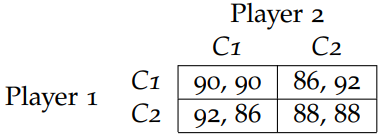
\includegraphics[width=0.3\textwidth]{nash_pareto}\\
    $(88, 88)$ is a Nash equilibrium, whereas the 3 others options are Pareto optimal.
\end{table}

\subsubsection{Social optimality}

\begin{itemize}
\item A choice of strategies (one by each player) is \textit{socially optimal} if it maximizes the sum of the players' payoff.
\item It is also Pareto optimal.
\end{itemize}

\section{Summary}

\begin{figure}[H]
    \centering
    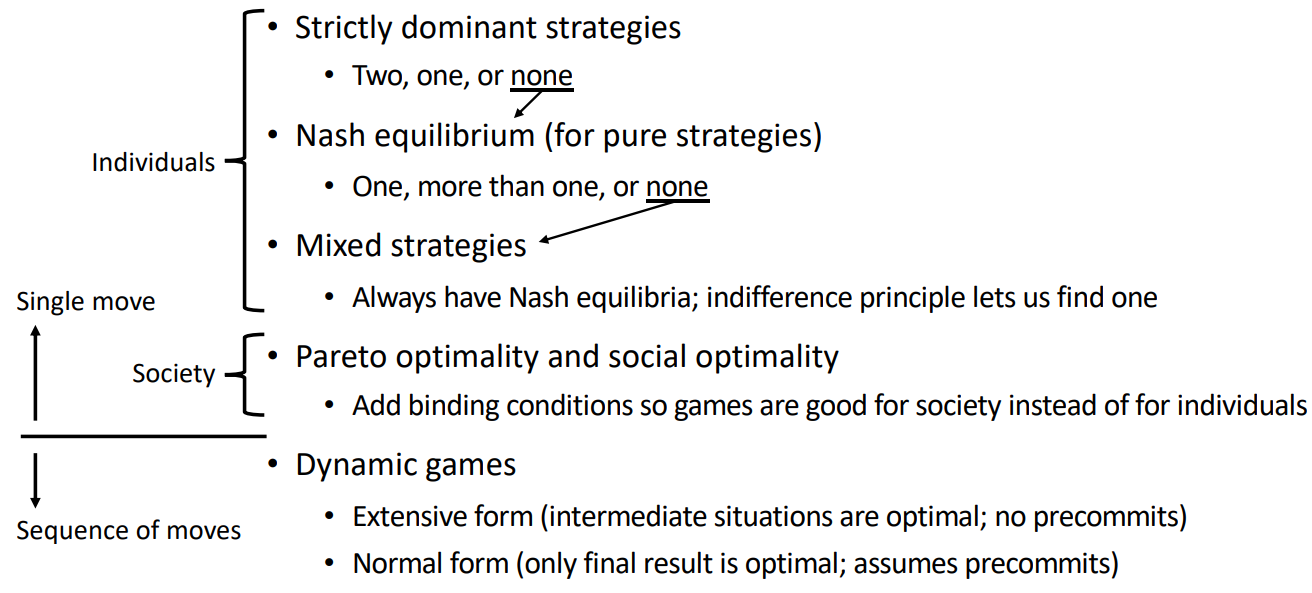
\includegraphics[width=0.8\textwidth]{game_theory_sum}
\end{figure}

